\documentclass{beamer}
\usepackage{graphicx}
\def \sarccontrib {{\bf SARC contribution}}
\newsavebox\myv

\begin{document}
\title{Optimizing the software stack of a cosmic proportions cluster of multi-core machines}
\author{Sebastian Pop}
\institute{SARC: Samsung Austin R\&D Center}
\date{February 5, 2017}

\frame{\titlepage}

\frame{\frametitle{Android: a Cosmic Size Cluster}
  \begin{itemize}
  \item top500: $10M$ cores / $15.3MW$ \footnote{\url{https://www.top500.org/lists/2016/11}} / US$\$273$ million \footnote{\url{https://en.wikipedia.org/wiki/Sunway_TaihuLight}}
  \item Android devices: $\sim{}6B$ cores \footnote{4 cores / device} / $\sim{}300MW$ \footnote{battery $13.2Wh = 4.4V * 3000 mAh$, charging every 48 hours} / $\sim{}$US\$0
  \includegraphics[width=8cm]{active-devices.png}
  \end{itemize}
}

\frame{\frametitle{Android Open Source Project (AOSP) Software Stack}
  \begin{itemize}
  \item<1-> AOSP: common base for Android devices (+ customization)
  \item<1-> C/C++ for the platform libraries, Java for user interface
    {\small \begin{tabular}{c c c}
      ansic & 22 MLoC & 39\% \\
      cpp   & 13 MLoC & 23\% \\
      java  & 10 MLoC & 17\% \\
    \end{tabular}}
  \item<1-> $\sim80\%$ execution cycles in C/C++, $\sim20\%$ in Java
  \item<2-> release/updates/deprecation ($5\sim6$ years) \\
    \includegraphics[width=8cm]{android-versions.png} \footnote{Data collected during a 7-day period ending on January 9, 2017.}
  \end{itemize}
}

\frame{\frametitle{Why Optimizing the Performance of Android?}
  \onslide<1-> {
    Why bothering?
    \begin{itemize}
    \item the code of Android is cold (flat profile), full of branches
    \item there are few loops (image processing, compression, etc.)
    \end{itemize}
  }
  \vspace{.3cm}
  \onslide<2-> {
    Motivation:
    \begin{itemize}
    \item same code executed billions of time
    \item outer loop is outside the device
    \item profile how often code is in use
    \item variation over time following popularity of apps
    \item continuously monitor usage patterns
    \item tune code optimization over time
    \end{itemize}
    \vspace{.3cm}
    \begin{tabular}{c c c}
      $\$0.30$ / device / year & $\longrightarrow$ & $\$300M$ / billion devices / year \footnote{$\$0.12/kWh$, battery $13.2Wh = 4.4V * 3000 mAh$, charging every 48 hours} \\
      \includegraphics[width=1.5cm]{1watt.jpg} & & \includegraphics[width=3cm]{1GWatt.jpg}
    \end{tabular}
  }
}

\frame{\frametitle{Agenda}
  \begin{itemize}
  \item tools for performance analysis
  \item improve performance of AOSP libraries
  \item enable continuous profiling and optimization (AutoFDO)
  \item enable more secure execution environments (CFI)
  \end{itemize}
}

\frame{\frametitle{Performance Analysis}
  \begin{itemize}
  \item benchmarks: track performance over time (compiler/libraries)
  \item Linux perf: profile of cycles (per function, hot-spots)
  \item Valgrind: number of executed instructions (branches, R/W)
  \item static profiles: how many uses for a function
  \end{itemize}
}

\frame{\frametitle{Benchmarks}
  track performance (compiler/libraries) over time \\
  \includegraphics[width=11cm]{benchmarks.png}  
}

\frame{\frametitle{Benchmarks}
  on a real device (and a noisy benchmark...)
  \includegraphics[width=11cm]{benchmarks-device.png}
}

\frame{\frametitle{Performance Analysis with Valgrind}
  \begin{itemize}
  \item {\ttfamily valgrind [--tool=memcheck]} \\
    valgrind mostly known for its memory leak checker
  \item {\ttfamily valgrind --tool=cachegrind}
    \begin{itemize}
    \item cache and branch simulator
    \item count read, write, and branch instructions
    \item \sarccontrib{:} diff tool for cachegrind profiles \footnote{\url{https://github.com/bmrzycki/cg_difftext}}
    \end{itemize}
  \item {\ttfamily valgrind --tool=callgrind}
    \begin{itemize}
    \item execution call graph
    \item visualization tool kcachegrind
    \end{itemize}
  \end{itemize}
}

\begin{frame}[fragile]{Valgrind: Example -- SQLite}
  \begin{lrbox}{\myv}
    \begin{minipage}{\textwidth}
\begin{verbatim}
$ valgrind --tool=cachegrind ./sqlite_llvm <test.sql >/dev/null
[...]
--------------------------------------------------------------------------------
           Ir       I1mr   ILmr          Dr      D1mr    DLmr          Dw      D1mw    DLmw
--------------------------------------------------------------------------------
1,278,771,731 29,231,219 35,783 359,414,267 6,707,514 528,920 197,515,528 2,594,262 171,968  PROGRAM TOTALS
 
--------------------------------------------------------------------------------
         Ir      I1mr  ILmr         Dr      D1mr    DLmr         Dw    D1mw   DLmw  file:function
--------------------------------------------------------------------------------
363,052,233 7,560,087 3,122 97,707,865 1,084,529  77,197 44,505,055 217,826 29,838  src/sqlite3.c:sqlite3VdbeExec
 95,048,357    80,721   111 33,248,107    59,086   7,273 20,173,275      91      7  src/sqlite3.c:vdbeRecordCompareWithSkip
 68,045,026   695,509 1,144 14,883,933   114,698   1,918  5,525,733 272,507 19,249  src/sqlite3.c:balance
 56,713,554 1,101,002   276 18,416,705   683,914  21,085  3,453,665   1,947     25  src/sqlite3.c:sqlite3BtreeMovetoUnpacked
 45,344,891    59,660    66 13,589,490    66,121  18,775 12,795,281  59,451     86  src/sqlite3.c:sqlite3VdbeRecordUnpack
 36,550,248    47,192    94  9,615,816   217,845  11,567          0       0      0  src/sqlite3.c:cellSizePtr
 35,156,491 1,031,905   859  7,810,853   489,509   1,936  6,546,085 175,469 26,159  /build/glibc-2.19/malloc/malloc.c:_int_malloc
 34,402,967   219,015    40 12,316,213    31,625   1,007          0       0      0  src/sqlite3.c:vdbeRecordCompareInt
 31,287,698   269,233   121 10,094,976   398,015  57,982 10,094,976 797,005 41,768  /build/glibc-2.19/string/../ports/sysdeps/aarch64/memcpy.S:memcpy
 30,895,222 1,055,479   718  3,990,072    45,246     157  3,247,672   1,200     58  src/sqlite3.c:sqlite3VXPrintf
 29,633,734        87    87  6,992,348   510,654 147,437  1,945,350     292     14  src/sqlite3.c:vdbeSorterSort
 28,301,654 1,222,726   236  7,685,792   129,350     101  4,693,862  15,480     91  src/sqlite3.c:sqlite3BtreeInsert
 27,452,670   605,975   428  7,719,336   275,711   3,045  6,130,240   1,247    180  /build/glibc-2.19/malloc/malloc.c:_int_free
 26,152,338    93,230    53  5,107,641    26,455      59  3,502,857   6,705      2  src/sqlite3.c:sqlite3VdbeSerialGet
 21,638,172   664,339   241  7,621,765   197,153   7,033  5,509,634  12,988     53  src/sqlite3.c:sqlite3PagerAcquire
 19,904,842   811,018   134  6,875,142    93,695     809  4,223,778   6,655     72  src/sqlite3.c:insertCell
 17,184,877   622,046   254  5,927,277   207,045     101  3,228,818  13,564     78  src/sqlite3.c:pager_write
 16,511,495   127,072    29  5,189,327     7,164   1,105  2,358,785       0      0  src/sqlite3.c:serialGet
 14,566,464   347,254   101  5,076,192    68,798   4,135  3,972,672 131,226  9,179  src/sqlite3.c:moveToChild
 14,089,915   528,334   433  3,522,612   169,118     295      1,089      24     22  ???:???
 13,516,049   315,369    75  3,660,565    70,941     104  2,252,728   2,740     20  /build/glibc-2.19/malloc/malloc.c:malloc
 13,444,711   370,614    60  3,136,255    74,755  57,116  3,757,149       0      0  src/sqlite3.c:btreeParseCellPtr
 11,814,468   620,489   364  3,444,231   109,318     159  1,401,768  11,253      7  src/sqlite3.c:sqlite3VdbeHalt
  9,867,819   655,851   130  3,350,976    68,237      46  1,820,276  62,050     70  src/sqlite3.c:moveToRoot
  9,023,249   615,625   175  2,774,458    27,649      72  1,719,012     578      1  src/sqlite3.c:sqlite3VdbeMemGrow
  9,015,155   136,420   114  2,528,161    33,460      40  1,808,361      12      7  /build/glibc-2.19/nptl/pthread_mutex_lock.c:pthread_mutex_lock
  8,932,696   193,491    71  1,956,326    55,921      22  1,411,634       2      0  /build/glibc-2.19/nptl/pthread_mutex_unlock.c:__pthread_mutex_unlock_usercnt
  8,916,165    82,925    47  2,092,310         0       0  1,933,573   1,583      3  src/sqlite3.c:memjrnlWrite
  8,869,488   284,528    72  4,276,902   299,688   8,315  1,834,026   6,712     17  src/sqlite3.c:pcache1Fetch
  8,120,421   171,173   145          0         0       0  4,459,287 446,962 23,788  /build/glibc-2.19/string/../ports/sysdeps/aarch64/memset.S:memset
  7,759,659   338,888    58  2,364,882    24,321   1,308  1,624,112 104,416  1,631  src/sqlite3.c:sqlite3PcacheRelease
  6,799,934    97,805   282  2,068,211    38,793     684  1,555,697   3,672     11  src/sqlite3.c:sqlite3BtreeNext
  6,674,044    88,515   123  1,706,065     4,244      43  1,094,451       7      0  src/sqlite3.c:freeSpace
  6,536,765   760,083   320  2,119,849   121,314      85  1,091,200       0      0  src/sqlite3.c:sqlite3_step
\end{verbatim}
    \end{minipage}
  \end{lrbox}
  \resizebox{0.4\textwidth}{!}{\usebox\myv}
\end{frame}

\begin{frame}[fragile]{Valgrind: Example -- SQLite}
  \begin{lrbox}{\myv}
    \begin{minipage}{\textwidth}
\begin{verbatim}
$ cg_difftext.py cachegrind.out.gcc cachegrind.out.llvm
[file_a] cachegrind.out.gcc
[file_b] cachegrind.out.llvm
    Ir:      1,210,101,457      1,278,770,879  [        68,669,422]
  I1mr:         23,202,418         29,231,219  [         6,028,801]
  ILmr:             30,817             35,783  [             4,966]
    Dr:        337,329,529        359,414,081  [        22,084,552]
  D1mr:          6,107,672          6,707,514  [           599,842]
  DLmr:            522,450            528,920  [             6,470]
    Dw:        180,346,394        197,515,342  [        17,168,948]
  D1mw:          2,646,481          2,594,262  [           -52,219]
  DLmw:            172,947            171,968  [              -979]

[func] sqlite3VdbeExec
[file] src/sqlite3.c
    Ir:        305,641,560        363,052,233  [        57,410,673]
  I1mr:          4,725,208          7,560,087  [         2,834,879]
  ILmr:              2,215              3,122  [               907]
    Dr:         84,047,121         97,707,865  [        13,660,744]
  D1mr:            694,519          1,084,529  [           390,010]
  DLmr:             67,617             77,197  [             9,580]
    Dw:         29,174,474         44,505,055  [        15,330,581]
  D1mw:            170,442            217,826  [            47,384]
  DLmw:             29,600             29,838  [               238]
[...]
\end{verbatim}
    \end{minipage}
  \end{lrbox}
  \resizebox{0.5\textwidth}{!}{\usebox\myv}
\end{frame}

\frame{\frametitle{Performance Analysis with Linux Perf}
  Two modes of operation:
  \begin{itemize}
  \item sum up all counters: {\ttfamily perf stat}
  \item record events: {\ttfamily perf record}
  \end{itemize}
}

\begin{frame}[fragile]{Linux Perf: Example -- SQLite}
  \begin{lrbox}{\myv}
    \begin{minipage}{\textwidth}
\begin{verbatim}
  $ perf stat ./sqlite_llvm <test.sql >/dev/null
 
 Performance counter stats for './sqlite_llvm':
 
       1045.856070      task-clock (msec)         #    1.000 CPUs utilized
                 1      context-switches          #    0.001 K/sec
                 0      cpu-migrations            #    0.000 K/sec
               809      page-faults               #    0.774 K/sec
     1,636,720,010      cycles                    #    1.565 GHz                     [83.16%]
       548,530,227      stalled-cycles-frontend   #   33.51% frontend cycles idle    [83.16%]
       218,991,051      stalled-cycles-backend    #   13.38% backend  cycles idle    [67.04%]
     3,385,841,295      instructions              #    2.07  insns per cycle
                                                  #    0.16  stalled cycles per insn [83.54%]
       709,436,490      branches                  #  678.331 M/sec                   [83.54%]
         2,586,354      branch-misses             #    0.36% of all branches         [83.17%]
 
       1.045918998 seconds time elapsed
\end{verbatim}
    \end{minipage}
  \end{lrbox}
  \resizebox{0.5\textwidth}{!}{\usebox\myv}
\end{frame}

\frame{\frametitle{Static Profiles}
  \begin{itemize}
  \item information known at compile time
  \item decisions made by the compiler
    \vspace{1cm}
  \item -flto: static call-graph
  \item estimated frequencies per call / basic block
  \item -mllvm -stats
    \begin{itemize}
    \item register spills
    \item redundancies eliminated
    \item functions inlined
    \end{itemize}
  \end{itemize}
}

\frame{\frametitle{Improve performance of AOSP libraries}
  \sarccontrib{\bf s}
  \begin{itemize}
  \item update Android NDK libc++, make it easy to keep updated
  \item 20x speedup of std::string.find() in libc++ and libstdc++
    need to port perf to memmem and strstr of bionic and glibc
  \item improve perf of shared\_ptr in libc++
  \item improve perf of string to int value parsing in libc++
  \end{itemize}
}

\frame{\frametitle{Benchmarking Standard Libraries}
  \sarccontrib{:} std-benchmark\footnote{https://github.com/hiraditya/std-benchmark}
  \vspace{1cm}
  \begin{itemize}
  \item std-benchmark provides micro-benchmarks for functions in libc and C++ standard library
  \item detect room for improvement
    \begin{itemize}
    \item compile with different compilers
    \item link with different standard libraries
    \item run on different machines: CPUs, architectures
    \end{itemize}
  \end{itemize}
}

\frame{\frametitle{AutoFDO: Feedback Directed Optimization}
  \begin{itemize}
  \item Linux-perf extracts profiles of running systems
  \item little to no overhead \footnote{Google Wide Profiling: A Continuous Profiling Infrastructure for Data Centers, IEEE Micro (2010)}
  \item coverage (basic block frequencies) from dynamic profiles
  \item continuous profiling and tuning of optimizations
    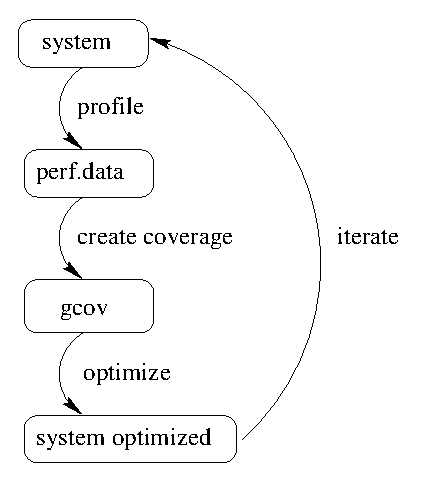
\includegraphics[width=5cm]{continuous-autofdo.eps}
  \end{itemize}
}

\frame{\frametitle{AutoFDO: Example}
  \includegraphics[width=11cm]{autofdo.eps}
}

\frame{\frametitle{AutoFDO: Code Optimizations}
  \begin{itemize}
  \item better inlining \footnote{Lightweight Feedback-Directed Cross-Module Optimization, CGO 2010}, devirtualization, function instantiation
  \item hot/cold code placement
  \item register allocation, jump-threading, etc.
  \end{itemize}
}

\frame{\frametitle{AutoFDO: More Precise Coverage}
  \begin{itemize}
  \item Intel-LBR (Last Branch Record): last 16 taken branches
  \item provides more precise basic block execution frequency
  \item how do we do this on ARM?
  \end{itemize}
}

\frame{\frametitle{ARM-ETM: Embedded Trace Macrocell}
  \begin{itemize}
  \item ARM-ETM: records execution traces (for debug)
  \item dedicated circular buffer 1 to 3MB ($\sim10^5$ branches/MB)
  \item no overhead
  \item support in Linux kernel by Mathieu Poirier (Linaro)
  \item next android kernel Linux-4.9 will support ARM-ETM
    \vspace{1cm}
  \item \sarccontrib{:} how to use ARM-ETM for AutoFDO
    \begin{itemize}
    \item perf-inject translates execution traces to LBR events
    \item patch similar to perf-inject for Intel Process Trace
    \end{itemize}
  \end{itemize}
}

\frame{\frametitle{AutoFDO: with ARM-ETM}
  \includegraphics[width=10cm]{autofdo-etm.eps}
}

\frame{\frametitle{From Dynamic Profiles to Power Usage}
  \begin{itemize}
  \item traditionally, per app battery usage (ammeter on wire) \footnote{An Analysis of Power Consumption in a Smartphone, USENIX'10}
    \vspace{1cm}
  \item Linux-perf profiles provide a more accurate picture
    \begin{itemize}
    \item profiles from the field: real world use-cases
    \item merge together different profiles
    \item compute code execution frequency
    \item power consumption estimation per line of code
    \end{itemize}
  \end{itemize}
}

\frame{\frametitle{Towards more secure devices}
  \begin{itemize}
  \item Control Flow Integrity (CFI): $2\%$ overhead \footnote{Enforcing Forward-Edge Control-Flow Integrity in GCC\&LLVM, USENIX'14}
  \item to enable on Android: need to further reduce its cost
  \end{itemize}
}

\end{document}
